% L14a figure: eigenvalues, eigenvectors, and the modes of x' = A x.
%
% Both panels use the eigenvectors v1 = (2, 1) and v2 = (-1, 1).
%   (a) A = [1.5 1; 0.5 1], eigenvalues 2 and 0.5. A stretches v1 and v2
%       along their own lines, A v1 = 2 v1 and A v2 = 0.5 v2, while the general
%       vector w = (-0.3, 1) turns to A w = (0.55, 0.85).
%   (b) A = [-1 1; 0.5 -1.5], eigenvalues -0.5 and -2. The initial state
%       x(0) = (0.4, 1.4) = 0.6 v1 + 0.8 v2 splits into two modes. At t = 1 the
%       modes are 0.6 exp(-0.5) v1 = (0.728, 0.364) and 0.8 exp(-2) v2 = (-0.108, 0.108),
%       and their sum is x(1) = (0.620, 0.472). The blue curve is the analytic
%       solution x(t) = 0.6 exp(-0.5 t) v1 + 0.8 exp(-2 t) v2.
%
% Drawn on November 19, 2026 with the palette and build of Fig-PhasePortraits.
% The notebook SVG carries a dark palette added by theme_svg.py; keep new colors
% in that script's mapping when changing the palette here.
\documentclass[tikz,border=4pt]{standalone}
\usepackage{amsmath}
\usepackage[no-math]{fontspec}
\IfFontExistsTF{Arial}{\setsansfont{Arial}}{\setsansfont{TeX Gyre Heros}}
\renewcommand{\familydefault}{\sfdefault}
\usetikzlibrary{arrows.meta, decorations.markings}

% Ink and blue match the L13a figures. Red marks eigenvectors, as in
% Fig-PhasePortraits; blue marks the general vector and the solution curve.
\definecolor{vnink}{HTML}{202124}
\definecolor{gdblue}{HTML}{0091FF}
\definecolor{evred}{HTML}{D93025}

\newcommand{\vv}[1]{\mathbf{v}_{#1}}

\tikzset{
  axis/.style={draw=vnink, line width=0.5pt, -{Stealth[length=2mm, width=1.6mm]}},
  eigline/.style={draw=evred, line width=0.9pt, dash pattern=on 4pt off 3pt},
  invec/.style={draw=vnink, line width=1.0pt, -{Stealth[length=2.6mm, width=2mm]}},
  outvec/.style={line width=2.0pt, -{Stealth[length=3.2mm, width=2.6mm]}},
  mode/.style={draw=evred, line width=1.4pt, -{Stealth[length=2.4mm, width=1.9mm]}},
  guide/.style={draw=vnink, line width=0.6pt, dash pattern=on 1pt off 2pt},
  flow/.style={draw=gdblue, line width=1.1pt, postaction={decorate},
    decoration={markings, mark=at position 0.3 with {\arrow[gdblue]{Stealth[length=2.6mm, width=2mm]}}}},
  lab/.style={text=vnink, font=\small, fill=white, inner sep=1.2pt},
  redlab/.style={text=evred, font=\small, fill=white, inner sep=1.2pt},
  bluelab/.style={text=gdblue, font=\small, fill=white, inner sep=1.2pt},
  title/.style={text=vnink, font=\sffamily\bfseries, align=center},
  sub/.style={text=vnink, font=\sffamily\small, align=center},
  dot/.style={fill=gdblue, draw=none},
}

\begin{document}
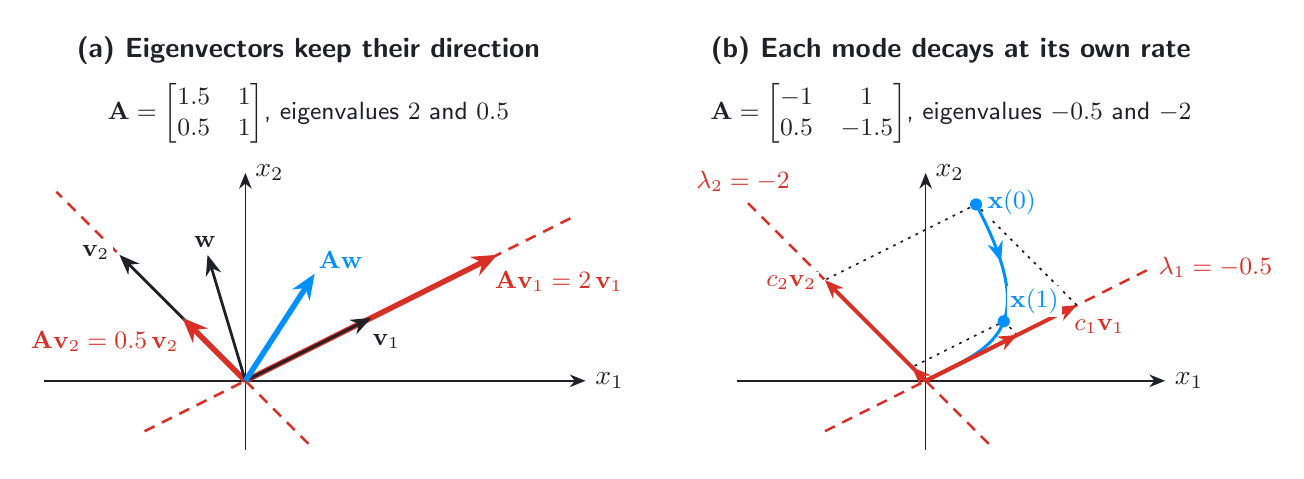
\begin{tikzpicture}[x=1.6cm, y=1.6cm]

% ------------------------------------------------------------ (a) A v = lambda v
\begin{scope}
  \node[title] at (0.5, 2.62) {(a) Eigenvectors keep their direction};
  \node[sub] at (0.5, 2.12) {$\mathbf{A}=\begin{bmatrix}1.5&1\\0.5&1\end{bmatrix}$, eigenvalues $2$ and $0.5$};
  \draw[axis] (-1.6, 0) -- (2.7, 0) node[right, text=vnink] {$x_1$};
  \draw[axis] (0, -0.55) -- (0, 1.65) node[right, text=vnink] {$x_2$};
  \draw[eigline] (-0.8, -0.4) -- (2.6, 1.3);
  \draw[eigline] (0.5, -0.5) -- (-1.5, 1.5);
  % longer vector first, so the shorter one stays visible on top
  \draw[outvec, draw=evred] (0, 0) -- (2, 1);
  \draw[invec] (0, 0) -- (1, 0.5);
  \draw[invec] (0, 0) -- (-1, 1);
  \draw[outvec, draw=evred] (0, 0) -- (-0.5, 0.5);
  \draw[invec] (0, 0) -- (-0.3, 1);
  \draw[outvec, draw=gdblue] (0, 0) -- (0.55, 0.85);
  \node[redlab, anchor=north west] at (1.95, 0.9) {$\mathbf{A}\vv{1}=2\,\vv{1}$};
  \node[lab, anchor=north west] at (0.98, 0.4) {$\vv{1}$};
  \node[lab, anchor=east] at (-1.05, 1.02) {$\vv{2}$};
  \node[redlab, anchor=north east] at (-0.5, 0.42) {$\mathbf{A}\vv{2}=0.5\,\vv{2}$};
  \node[lab, anchor=south] at (-0.32, 1.03) {$\mathbf{w}$};
  \node[bluelab, anchor=south west] at (0.55, 0.86) {$\mathbf{A}\mathbf{w}$};
\end{scope}

% ------------------------------------------------------------ (b) modes
\begin{scope}[shift={(5.4, 0)}]
  \node[title] at (0.2, 2.62) {(b) Each mode decays at its own rate};
  \node[sub] at (0.2, 2.12) {$\mathbf{A}=\begin{bmatrix}-1&1\\0.5&-1.5\end{bmatrix}$, eigenvalues $-0.5$ and $-2$};
  \draw[axis] (-1.5, 0) -- (1.9, 0) node[right, text=vnink] {$x_1$};
  \draw[axis] (0, -0.55) -- (0, 1.65) node[right, text=vnink] {$x_2$};
  \draw[eigline] (-0.8, -0.4) -- (1.8, 0.9);
  \draw[eigline] (0.5, -0.5) -- (-1.45, 1.45);
  \node[redlab, anchor=west] at (1.82, 0.9) {$\lambda_1=-0.5$};
  \node[redlab, anchor=south] at (-1.45, 1.47) {$\lambda_2=-2$};
  % the parallelograms that add the two modes, at t = 0 and t = 1
  \draw[guide] (1.2, 0.6) -- (0.4, 1.4) -- (-0.8, 0.8);
  \draw[guide] (0.7278, 0.3639) -- (0.6195, 0.4722) -- (-0.1083, 0.1083);
  % the solution curve
  \draw[flow] plot[domain=0:5, samples=150, variable=\t]
    ({1.2*exp(-0.5*\t) - 0.8*exp(-2*\t)}, {0.6*exp(-0.5*\t) + 0.8*exp(-2*\t)});
  % the modes, longer first
  \draw[mode] (0, 0) -- (1.2, 0.6);
  \draw[mode] (0, 0) -- (0.7278, 0.3639);
  \draw[mode] (0, 0) -- (-0.8, 0.8);
  \draw[mode] (0, 0) -- (-0.1083, 0.1083);
  \fill[dot] (0.4, 1.4) circle (2.2pt);
  \fill[dot] (0.6195, 0.4722) circle (2.2pt);
  \node[bluelab, anchor=west] at (0.46, 1.42) {$\mathbf{x}(0)$};
  \node[bluelab, anchor=south west] at (0.64, 0.5) {$\mathbf{x}(1)$};
  \node[redlab, anchor=north west] at (1.15, 0.52) {$c_1\vv{1}$};
  \node[redlab, anchor=east] at (-0.84, 0.78) {$c_2\vv{2}$};
\end{scope}

\end{tikzpicture}
\end{document}
